

%\subsection{Provisioning on demand}
As a central component of our autoscaling system, the Scaler component is responsible for triggering the scaling actions. It supports horizontal scaling as a technique to add and remove resources to an application. Horizontal scaling enables to create a cluster of virtual machines associated to one application, which size is dynamically adapted to the workload fluctuations by adding or removing resources to the cluster. Even though this scaling technique is commonly supported for the majority of resource provisioning systems~\cite{ali-eldin_2012,bunch_2012,urgaonkar_agile_2008}, our approach is able to use the resource heterogeneity of the cloud infrastructures to improve the efficiency of the scaling actions.

In order to decide when to trigger a scaling action, our system uses the following two methods: 

% On the other hand, in our system, vertical scaling enables to add or remove resources with high or less cpu and memory using \emph{service live migration}. Using this mechanism, the Scaler migrates the hosted service (web applications) from one virtual machine to another with a better hardware configuration. To reduce the degradations caused by this type of migration or by the booting time of the new machine, the Scaler checks the proper functioning of the new machine in order to release the older one.


\begin{itemize}

%\item \emph{Response time analysis:} A precise analysis of the monitoring data is crucial to minimize performance degradations that are sometimes omitted by traditional analytical methods such as the median, average or moving average. To extract precise information from the monitoring data  (e.g. response times) describing the performance behavior of an application, we decided to extend a known smoothing technique called \emph{Weighted Moving Average} (WMA). Using our extension for WMA, it analyzes the monitoring data associating weights in an increasing order giving more importance to the latest monitoring data; and second it increments the original weight value of each data-point that exceeds the performance requirements. By doing so, our system analyzes the monitoring data giving special importance to the data points on which SLO violations have occurred, and thereby is able to detect and avoid the maximum number of violations.

%The weight increment can be modified to raise the awareness of the system to SLO violations  (in our experiments we defined the weight increment as twice the original weight of each data-point).

\item \emph{Definition of a reactive threshold:} Additionally to the fixed SLO threshold pre-defined by the QoS requirements (maximum response time), our system also includes an extra threshold (based on these requirements) that will enable in advance to react against any traffic variation, minimizing the number of SLO violations, or under-utilization of the provisioned resources. %As illustrated in Figure~\ref{thr}, this reactive threshold specifies one upper and lower boundaries creating two head-rooms between them and the fixed threshold pre-defined by the user.

%\begin{figure}[t]
%  \begin{center}
%    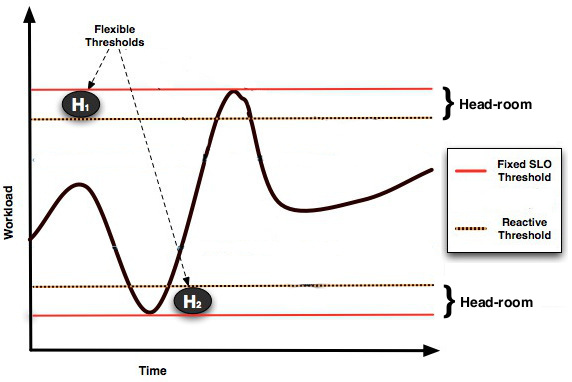
\includegraphics[width=.75\linewidth,height=3cm]{images/thresholdGraphic}
%  \end{center}
%\vspace{-3mm}
%  \caption{Reactive threshold.}
%  \label{thr}
%\end{figure}

\item \emph{Workload forecasting: }  The \emph{Predictor} component is utilized to trigger short-term forecast operations that will minimize the number of future SLA violations, as well as keeping a high level of efficiency in the predictions. 
\end{itemize}

Based on these techniques, the \emph{Scaler} evaluates whether the current performance behavior requires triggering any of the following scaling actions:

\begin{itemize}

\item \textbf{Scale out:} Additional resources are provisioned if the loaded system state (response time or CPU utilization) exceeds the upper threshold, and the \emph{Predictor} confirms that such traffic changes will remain at least during the next monitoring window. In our experiments, we define monitoring windows of 5 minutes as this interval is the minimum necessary time to collect fresh data from the monitoring engine provided by ConPaaS. 

\item \textbf{Scale back:} Resources are released if the loaded system state exceeds the lower threshold, and the \emph{Predictor} confirms that such traffic changes will remain at least during the next monitoring window.

\end{itemize}



%\subsubsection{Response time analysis - Time-series smoothing}

%When minimizing the SLA violations, a precise analysis of the monitoring data is crucial to improve the accuracy of the scaling decisions. It allows to %identify the resource requirements from the current workload type. This analyisis has even more importance when hosting web applications (e.g. %Wikipedia, Amazon) that need to provide high availability and performance to their clients. Moreover, the workload heterogeneity of this sites requires a %meticulous analysis of every monitoring data-point to reduce at the maximum the number of SLO violations. 

%\begin{figure}[htb]
%	\begin{minipage}[b]{0.49\linewidth}
%		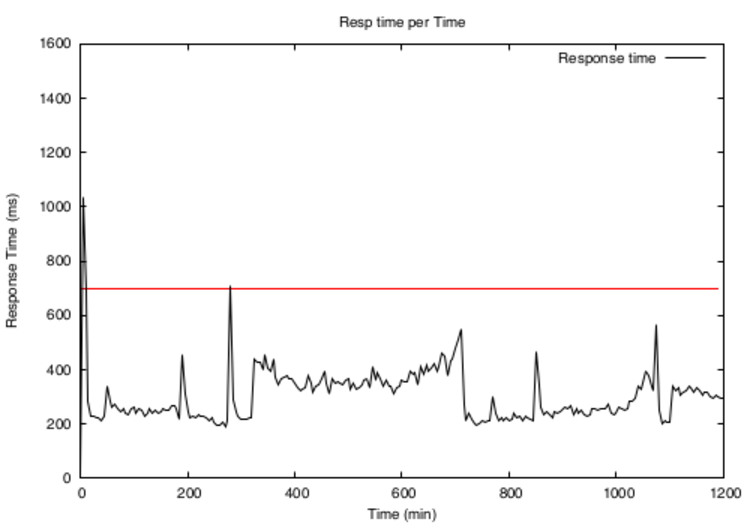
\includegraphics[width=4cm,height=3cm]{images/data2007/proxy_outputAvg.pdf}	
%		\vspace{-4mm}
%	\end{minipage}
%	\hfill
%	\begin{minipage}[b]{0.49\linewidth}
%		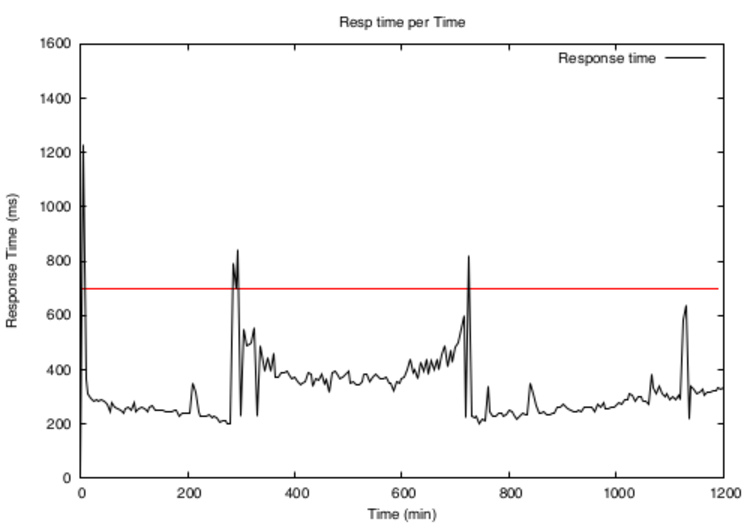
\includegraphics[width=4cm,height=3cm]{images/data2007/proxy_outputWMA.pdf}
%		\vspace{-4mm}
%	\end{minipage}
%\caption{Response times for a trace: Average vs extended WMA.}
%\label{fig:data_analysis}
%\end{figure}

%To obtain precise information (response times) that reflects the performance behavior of an application, we decided to extend a known smoothing technique called \emph{Weighted Moving Average} (WMA). This technique is widely used in resource provisioning systems instead of others such as the median, average or moving average. Using our extension of WMA, it first associated weights in an increasing order giving more importance to the latest monitoring data; and second it doubles the original weight value of each data-point that exceeds the performance requirements (response time). By doing so, the Scaler analyzes the monitoring data giving special importance to the data points on which SLO violations have occurred, and thereby being able to detect and avoid the maximum number of violations. As an example, Figure~\ref{fig:data_analysis} shows how several SLO violantions are omitted when analyzing the monitoring data using an average analytical method (left) than when using our version of WMA (right).

%\subsubsection{Definition of a reactive threshold}

%\fixme{Perhaps, you may want to omit this subsection, as it is more related to When to provision than How to provision ?}

%Initially, the user defines several performance requirements that will be utilized by the Scaler to trigger scaling actions. As we mentioned, these QoS goals are previously specified in the Service Level Objective (SLO). In particual, when hosting web applications, these performance requirements are usually related to the maximum processing time needed to serve any request (response times). Regarding SLO fulfillment the majority of resource provisioning system aims to maintain the processing time as closer as possible to the performance requirements. However, this operation can become a problem, as provisioning systems are vulnerable to temporal traffic oscillations causing SLO violations.

%Therefore, and based on the requirements, the Scaler defines a reactive threshold that will enable in advance to react against any traffic oscillation minimizing the number of SLO violations or period of time under-utilization of the provisioned resources. As shown in Figure~\ref{threshold}, this reactive threshold specifies one upper and lower boundaries creating two head-rooms between them and the performance requirements pre-defined by the user (for the response time). In the future, these two boundaries could be adjusted depending on the hardware configuration of each provisioned vm, as introduced in~\cite{beloglazov_adaptive_2010}.  


%\begin{figure}[htb]
 % \begin{center}
  %  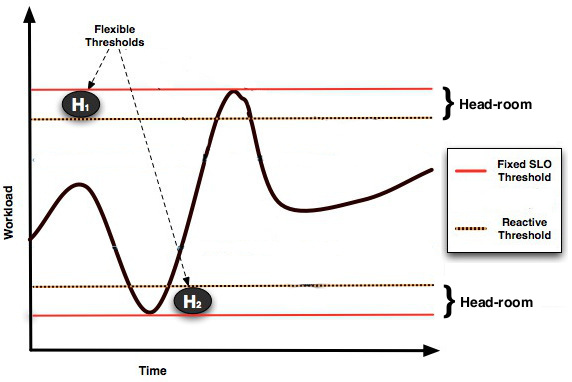
\includegraphics[width=.85\linewidth]{images/thresholdGraphic.jpg}
 % \end{center}
%\vspace{-5mm}
%  \caption{Reactive threshold.}
%  \label{threshold}
%\end{figure}



%\subsection{Online profiling of allocated instances\label{profiling}}
%\subsection{Measuring VM instance performance via online profiling\label{profiling}}

\subsection{Measuring VM instance performance \label{profiling}}

%Regarding resource heterogeneity of cloud infrastructures, a sensitivity analysis of the allocated resources is crucial to provide accurate scaling decisions. Accordingly, online profiling-based techniques~\cite{kaviani_profiling-as--service:_2011} have recently emerged as a solution to  estimate the resource's throughput under a certain workload. Traditionally, this technique replicates at runtime, a server hosting an application, with a new server with profiling instrumentation. To obtain  the profiling data, this new server analyzes the performance behavior of a specific resource under a fixed percentage of the incoming traffic~\cite{dejavu2012,jiangThesis}. The use of fixed workload to calculate the maximum throughput of a resource do not necessary imply the definition of more accurate profiles. A reason seems to be the lack of ideal performance isolation in cloud infrastructures which affects the precision of the definition of profiles, and consequently reduces the accuracy of the scaling decisions. Furthermore, setting a profiling environment, in a heterogeneous cloud infrastructure, requires as many additional resources as number of available configurations increasing the financial cost of this approach. 

 %To obtain  the profiling data, this new server analyzes the performance behavior of a specific resource under a fixed percentage of the incoming traffic~\cite{dejavu2012,jiangThesis}. The use of fixed workload to calculate the maximum throughput of a resource do not necessary imply the definition of more accurate profiles. A reason seems to be the lack of ideal performance isolation in cloud infrastructures which affects the precision of the definition of profiles, and consequently reduces the accuracy of the scaling decisions.

Even though the use of \emph{online} profiling techniques is still under study, the use of synthetic workload, the configuration of a parallel environment and the heterogeneity of the cloud resources are the major drawbacks for its adoption. These techniques increase the operational cost and do not necessarily improve the accuracy of the scaling decisions. As a consequence, to address these drawbacks we designed a novel online profiling technique that gives an estimation of the optimized throughput of each allocated VM instance type without the need for additional resources or parallel environments. To do that, the \emph{Profiler} component uses the provisioned resources and the real workload for the analysis and estimation of the computing capacity of each available server configuration.

%Even though the use of online-profiling techniques is still under study, the configuration of a parallel %environment and the limited accuracy of its scaling decisions are the major drawbacks for its %adoption.



%Cpu.usage is relative to nominal frequency of the CPU’s – not the amount of time the CPU was busy, which is generally more relevant.

\begin{algorithm}
{\scriptsize
\SetAlgoLined
\SetInd{0mm}{2mm}
\KwData{ \\Service Level Objective, \emph{slo} \\ List of allocated VM instance types, \emph{inst\_types} \\ Compute units per \emph{inst\_type}, \emph{compute\_units$_{inst}$}}

\KwResult{VM instances performance classification, \emph{list\_perf}}

\While{ allocated instances to profile}{
\BlankLine
Collect profiling data of \emph{inst\_type}: \emph{req\_rate, \%cpu\_usage and resp\_time}\;

\While{ profiling data to smooth}{  \label{alg:smooth}
// Perform smoothing percentiles technique \;
\If{ \emph{resp\_time}$_i$ $>$ (slo * 0.25) and \emph{resp\_time}$_i$ $<=$ (slo * 0.75)}{ 
	\If{ \emph{req\_rate}$_i$ $>$ 0 and \emph{\%cpu\_usage}$_i$ $<$ 75}{ 
		\hspace{3mm} Add \emph{\%cpu\_usage$_i$} to \%cpu\_usage\_data\;
		\hspace{3mm} Add \emph{req\_rate$_i$} to req\_rate\_data\;
		\hspace{3mm} Add \emph{resp\_time$_i$} to resp\_time\_data\;
}
}
} \label{alg:endSmooth}
\BlankLine
Initialize instance capacity \emph{Ideal\_Throughput$_{inst}$} to 0 \;
\uIf{ \emph{resp\_time\_data}, \emph{\%cpu\_usage\_data}, \emph{req\_rate\_data}  \textbf{not empty}}{
Calculate average of \emph{\%cpu\_usage\_data}, \emph{\%CPU\_usage$_{inst}$} \; \label{alg:throughput_start}
Calculate average of \emph{req\_rate\_data}, \emph{Num\_requests$_{inst}$} \;
\BlankLine
\emph{Ideal\_Throughput$_{inst}$} = $\dfrac{ \bigg( \dfrac{\emph{\%CPU\_usage$_{inst}$} } {100} \bigg)} {\emph{Num\_requests$_{inst}$ } }$  \; \label{alg:throughput_end}
\BlankLine
Store instance computing capacity, \emph{Ideal\_Throughput$_{inst}$} \; 
}
\Else{ 
	Use historic value of \emph{Ideal\_Throughput$_{inst}$} for \emph{inst\_type}\;
}
\BlankLine
// Classify \emph{inst\_type} based on its computing capacity \; \label{alg:clas}
\If{ Ideal\_Throughput$_{inst}$ == 0 }{
Use \emph{compute\_units$_{inst}$} of \emph{inst\_type} to rank \emph{inst\_type} in \emph{list\_perf}\;
}
\Else{ 
Use new value of \emph{Ideal\_Throughput$_{inst}$} to rank \emph{inst\_type} in \emph{list\_perf}\; \label{alg:end_clas}
}
}
}
\caption{VM instance profiling algorithm}
\label{profilingAlg}
\end{algorithm}

As detailed in Algorithm~\ref{profilingAlg}, once the \emph{Scaler} component decides to trigger a scaling action, the \emph{Profiler} component estimates the throughput of the allocated instances according to the following steps:



\paragraph{Collection of monitoring data} It collects the latest hour of monitoring data from each VM instance type. This data contains information about monitoring metrics such as the request rate, total percentage of cpu usage and response time, which provide enough feedback for the definition of instance profiles. In fact, when provisioning web applications, these metrics are commonly used to decide whether to trigger scaling actions or not \cite{smartscale_2012,urgaonkar_agile_2008}. Nevertheless, other metrics such as the network bandwidth and memory usage can also be collected to define instance profiles.


\paragraph{Data smoothing} The \emph{Profiler} performs a smoothing technique over the profiling data of each instance to remove the noise generated by traffic spikes. As pointed out in~\cite{gandhi_hybrid_2012}, when hosting web applications sudden changes in the workload, interference due to virtualization or OS activities may affect the precision of the profiling process. Hence, we decided to smooth the profiling data during the latest hour (or older if there is not enough data) to identify the performance capacity of each allocated VM instance type. This technique allows to identify the optimized throughput of each instance while enforcing the performance requirements and avoiding CPU saturation. In particular, the \emph{Profiler} extracts the smoothed 75th and 25th percentiles from the response times below the SLO in correspondence with the \emph{reactive threshold}; and 75th percentile from the percentage of cpu usage data-points. (See Lines \ref{alg:smooth}-\ref{alg:endSmooth}). Note that, we only use the 75th percentile from the cpu usage due to lower values in the cpu usage do not imply a system free of SLA violations. As an example, \emph{m1.small} instances can throw violations even under percentages of cpu usage lower than 25\%. 

% Why these percentiles

%As an example in Figure~\ref{fig:vm_performance1} and Figure~\ref{fig:vm_performance2}, we show the profiling data and percentiles for one "m1.small" and one "c1.medium" EC2 instance types during one hour. The gray areas represent the ranges of response times and cpu usage comprised by the percentiles. Red circles contain all data points that will be used to calculate the optimized throughput of one VM instance. As we mentioned above, some data points are excluded as they identify periods of time on which resources suffered from under-utilization or over-utilization (denoted by white areas). Furthermore, as shown in Figure~\ref{fig:vm_performance1}, a short number of data points are comprised between the percentiles for the "m1.small" instance. Its poor hardware configuration makes this instance type more vulnerable to sudden changes in the workload.

Figure~\ref{fig:vm_performance1} shows the profiling data and percentiles for one "m1.small" EC2 instance type during one hour. The gray areas represent the ranges of response times and cpu usage comprised by the percentiles. Red circles contain all data points that will be used to calculate the optimized throughput. In Figure~\ref{fig:vm_performance1}, some data points are excluded as they identify periods of time on which resources suffered from under-utilization or over-utilization (denoted by white areas). Similarly, a short number of data points are comprised between the percentiles for the "m1.small" instance. Its poor hardware configuration makes this instance type more vulnerable to sudden changes in the workload.

%and three red circles highlight several data-points on which the performance of the instance was optimal while enforcing the %SLO.

%\begin{figure*}[htb]
%	\begin{minipage}[b]{0.5\linewidth}
%		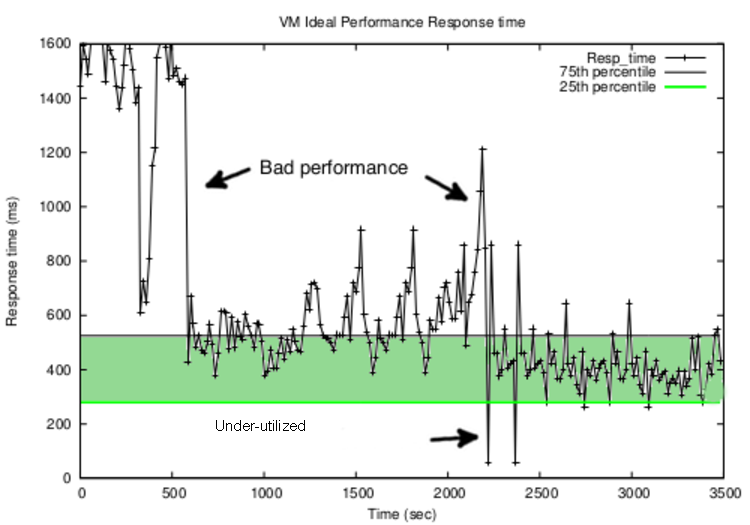
\includegraphics[height=4.5cm]{images/vm_performance_resp_smallEC2Remark.pdf}		%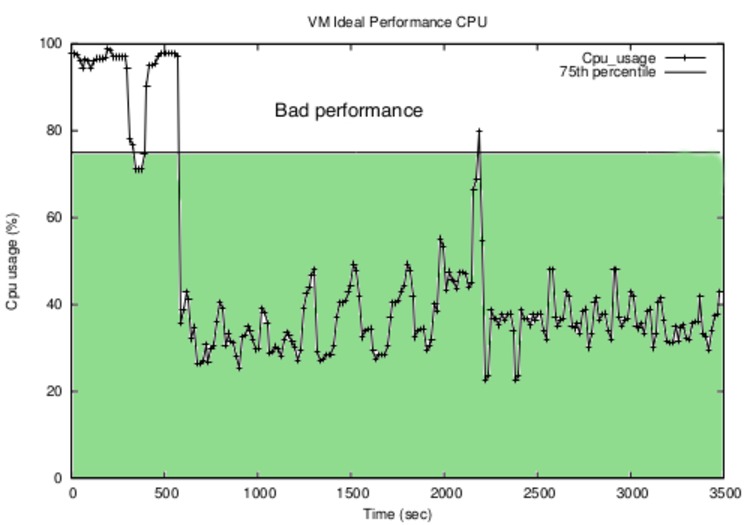
\includegraphics[height=4.5cm]{images/vm_performance_cpu_smallEC2Remark.pdf}
%		\vspace{-4mm}
%	\end{minipage}
%	\hfill
%	\begin{minipage}[b]{0.5\linewidth}
%		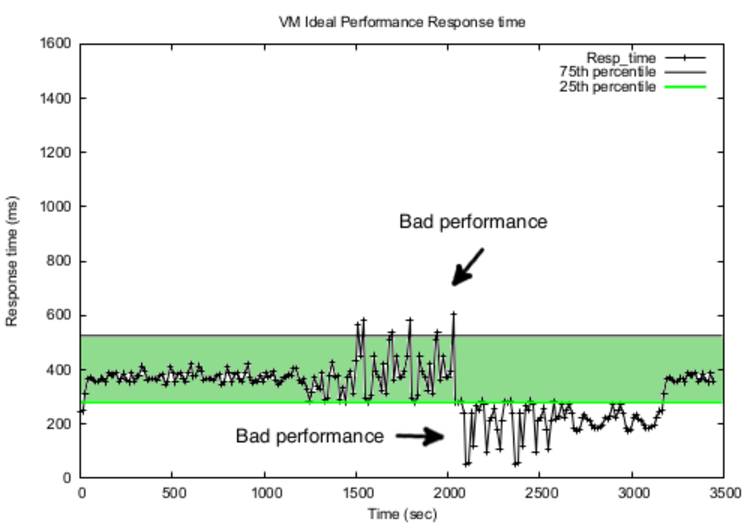
\includegraphics[height=4.5cm]{images/vm_performance_resp_c1mediumRemark.pdf}		%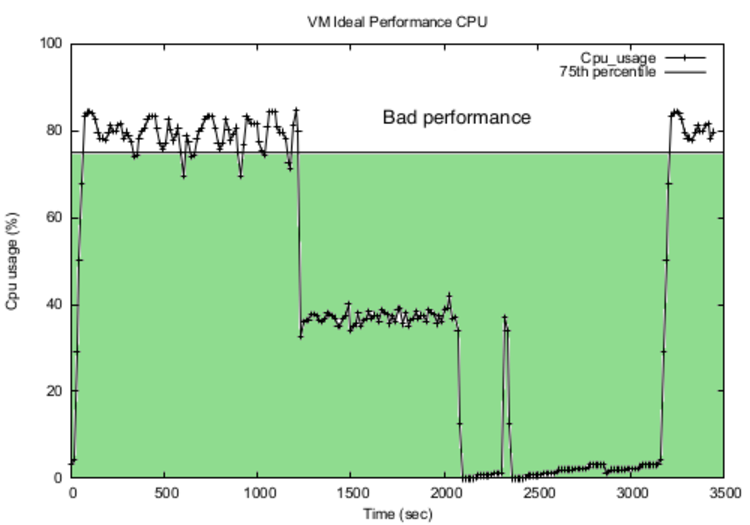
\includegraphics[height=4.5cm]{images/vm_performance_cpu_c1mediumRemark.pdf}
%		\vspace{-4mm}
%	\end{minipage}
%\caption{Profiling data and percentiles of m1.small and c1.medium EC2 instances.}
%\label{fig:vm_performance}
%\end{figure*}

\begin{figure}[t]
  \begin{center}
    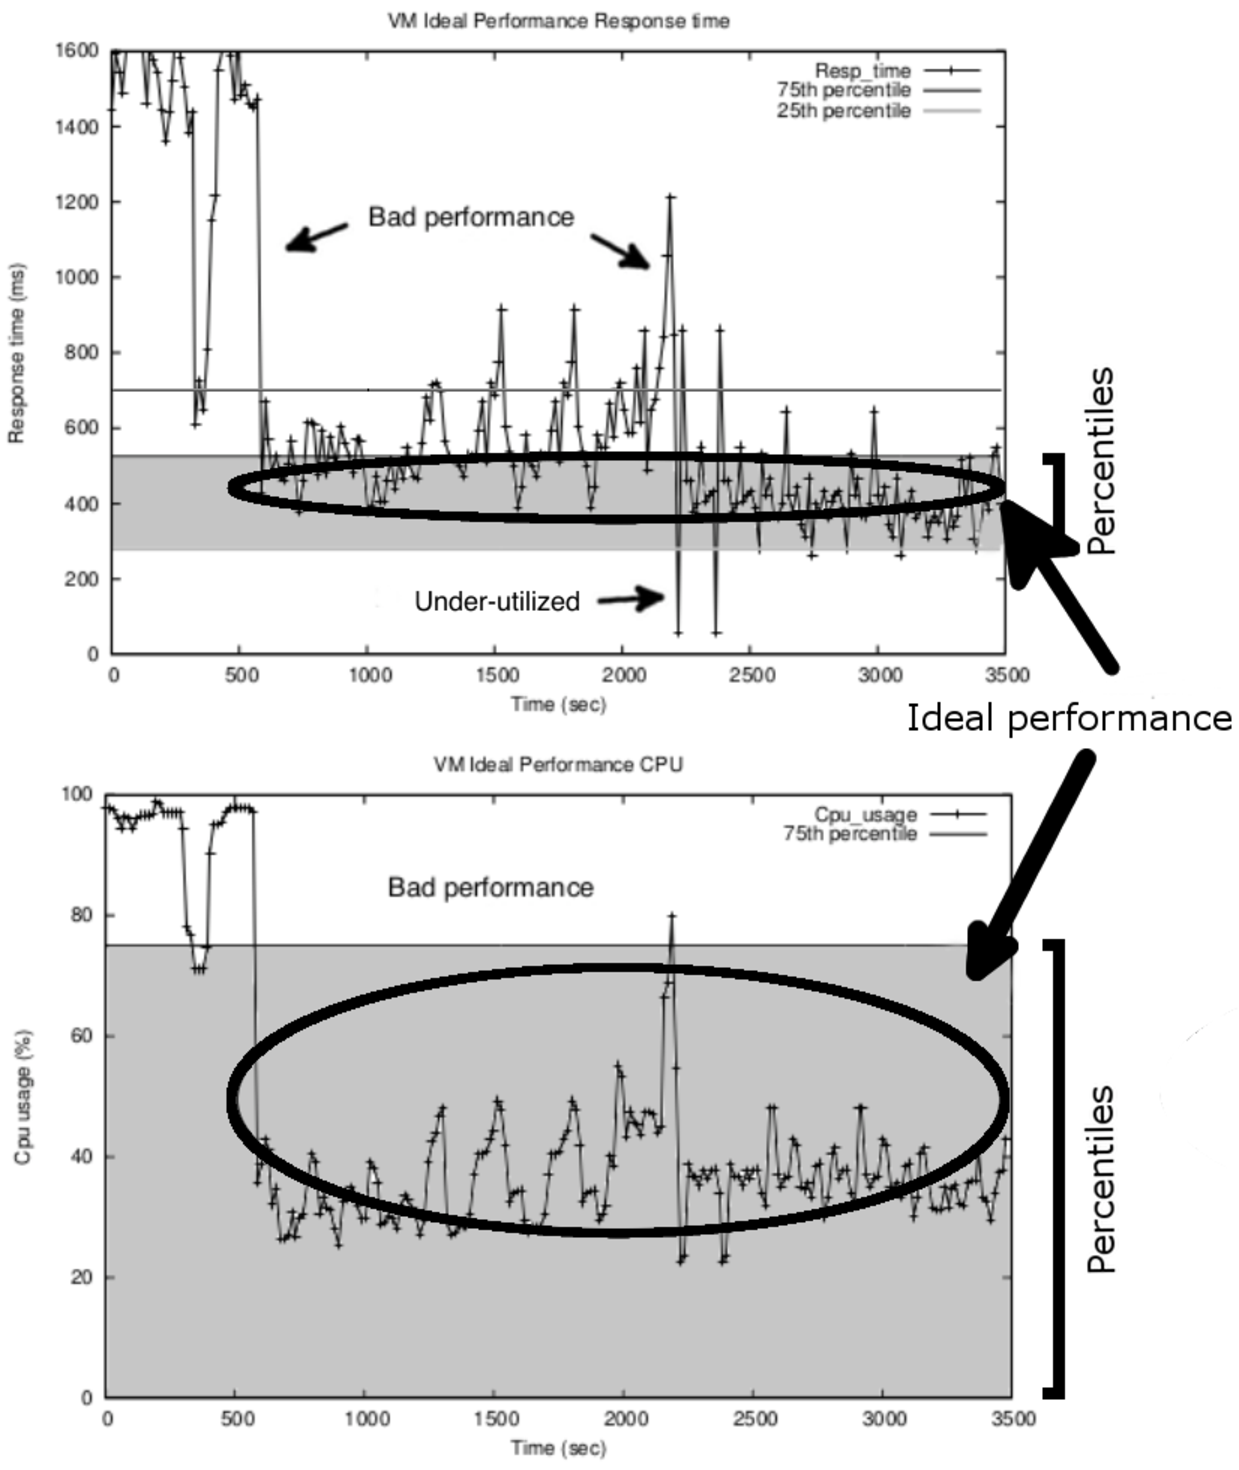
\includegraphics[width=0.8\linewidth, height=5.5cm]{images/idealSmallRemark.pdf}
  \end{center}
\vspace{-3mm}
  \caption{Profiling data and percentiles of m1.small.}
  \label{fig:vm_performance1}
\end{figure}

%\begin{figure}[t]
 % \begin{center}
  %  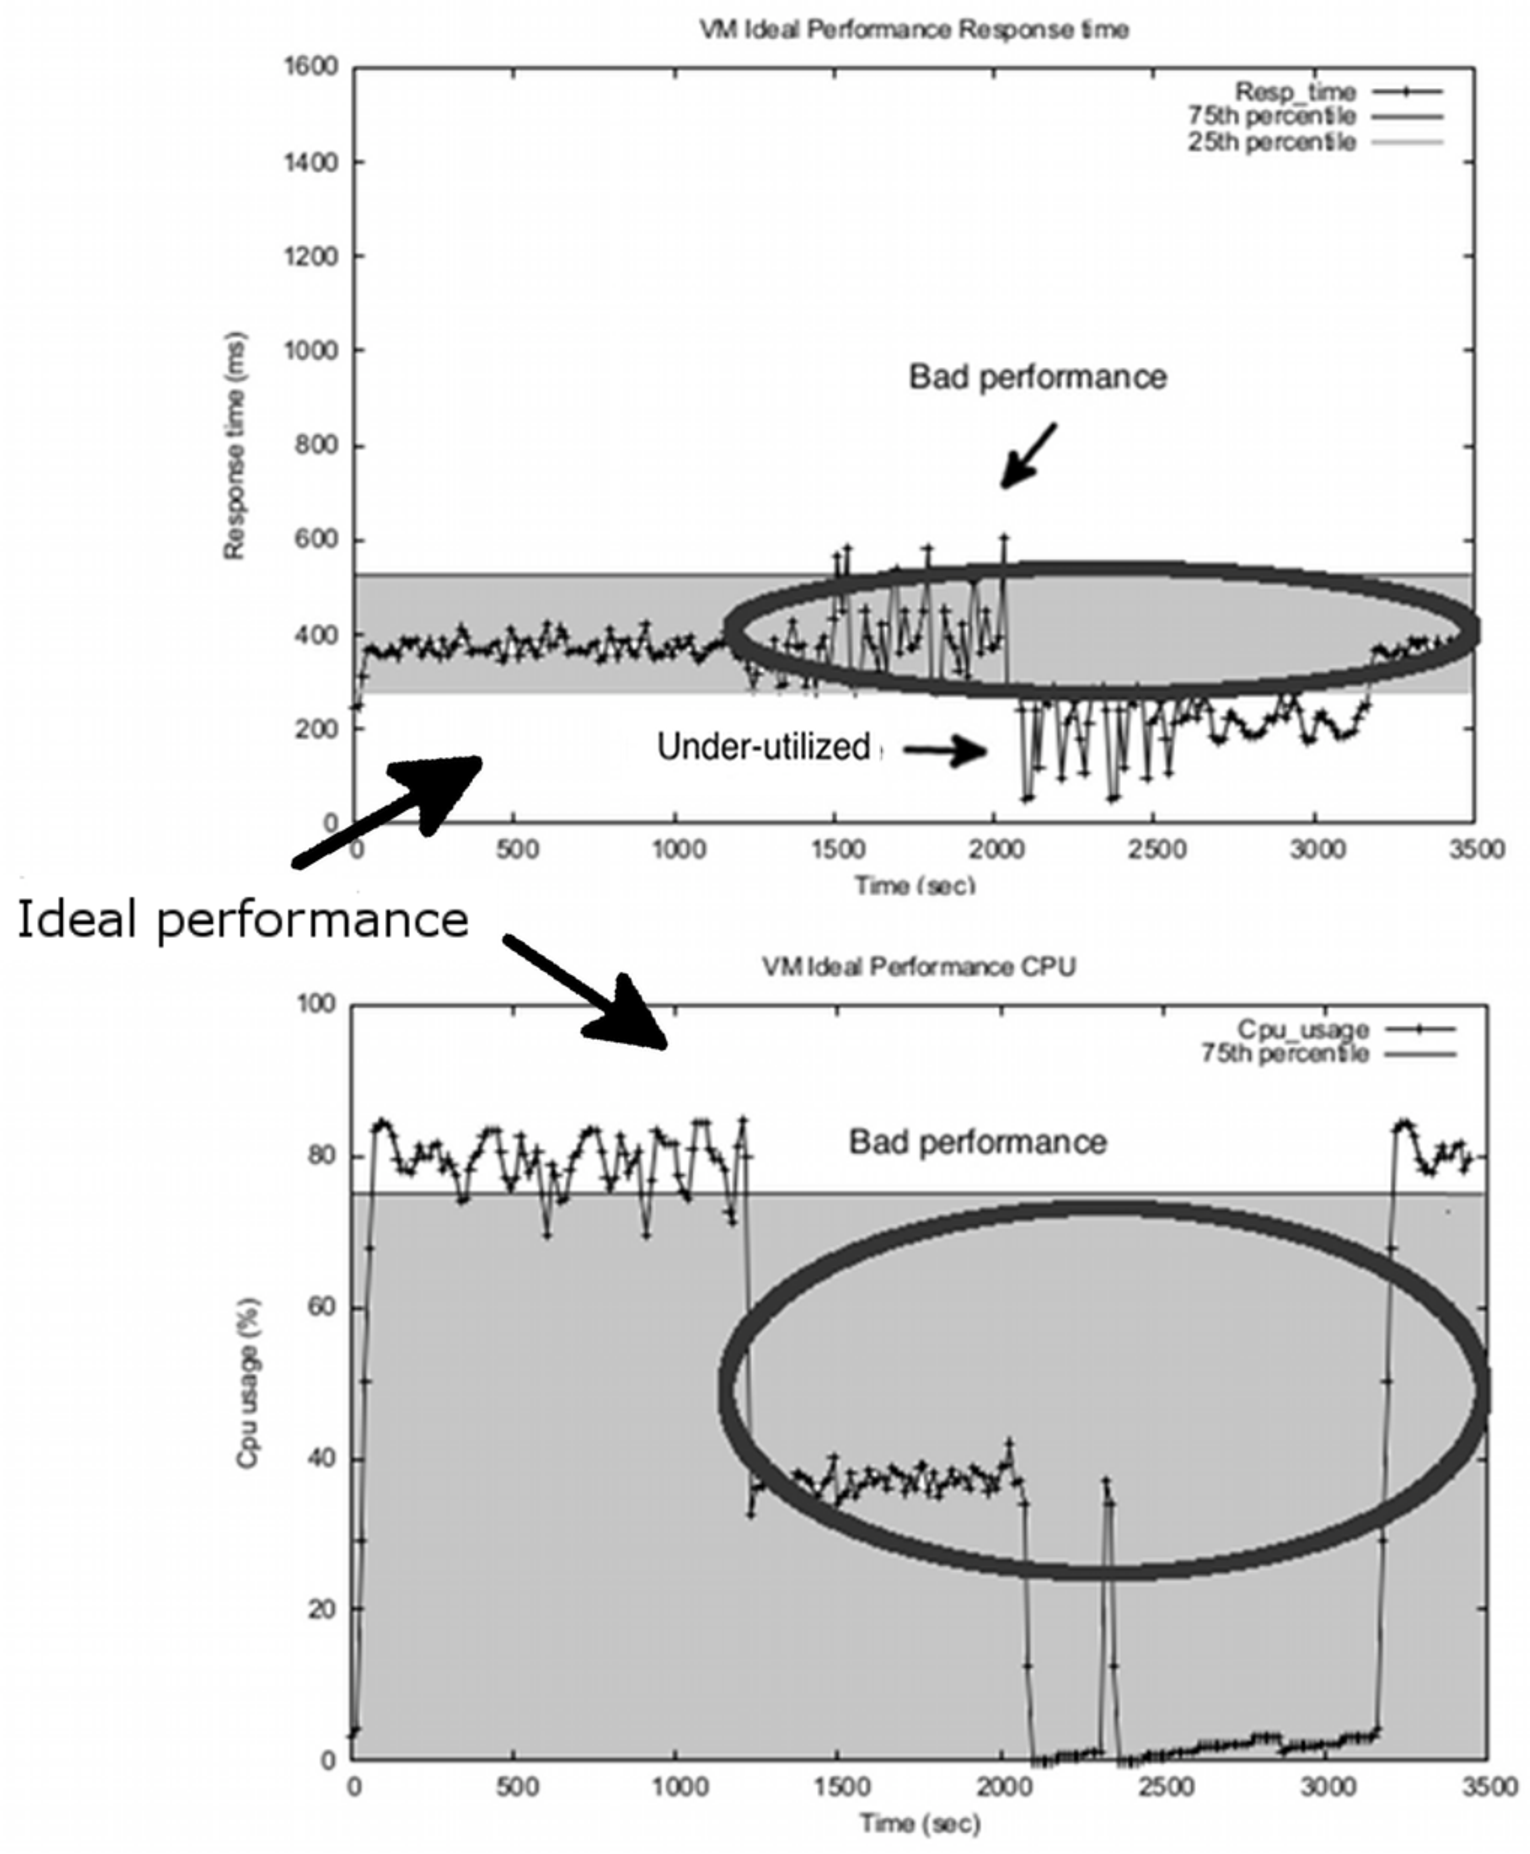
\includegraphics[width=0.8\linewidth, height=5cm]{images/idealc1MediumRemark.pdf}
 % \end{center}
 % \caption{Profiling data and percentiles of c1.medium.}
 % \label{fig:vm_performance2}
%\end{figure}

%\begin{figure*}[htb]
%	\begin{minipage}[b]{0.45\linewidth}
%		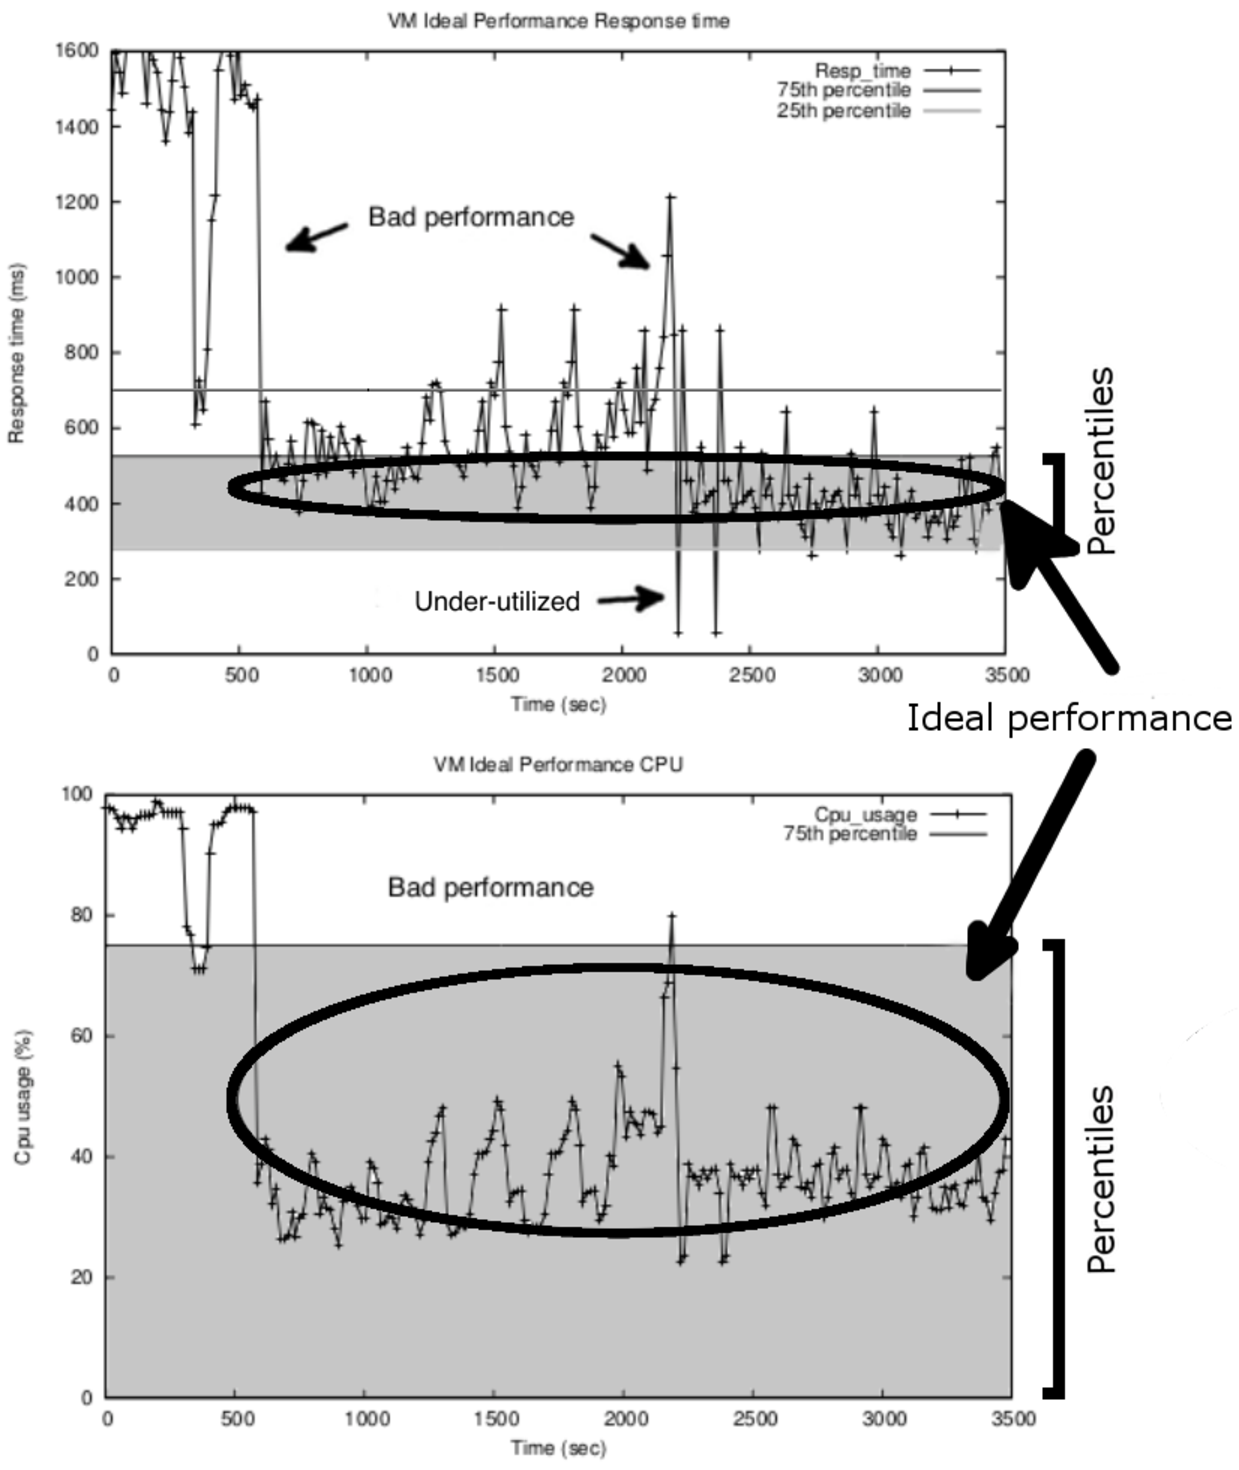
\includegraphics[height=8.5cm]{images/idealSmallRemark.pdf}		
%		\captionof*{figure}{ \textbf{m1.small}}	
%		\vspace{-4mm}
%	\end{minipage}
%	\hfill
%	\begin{minipage}[b]{0.45\linewidth}
%		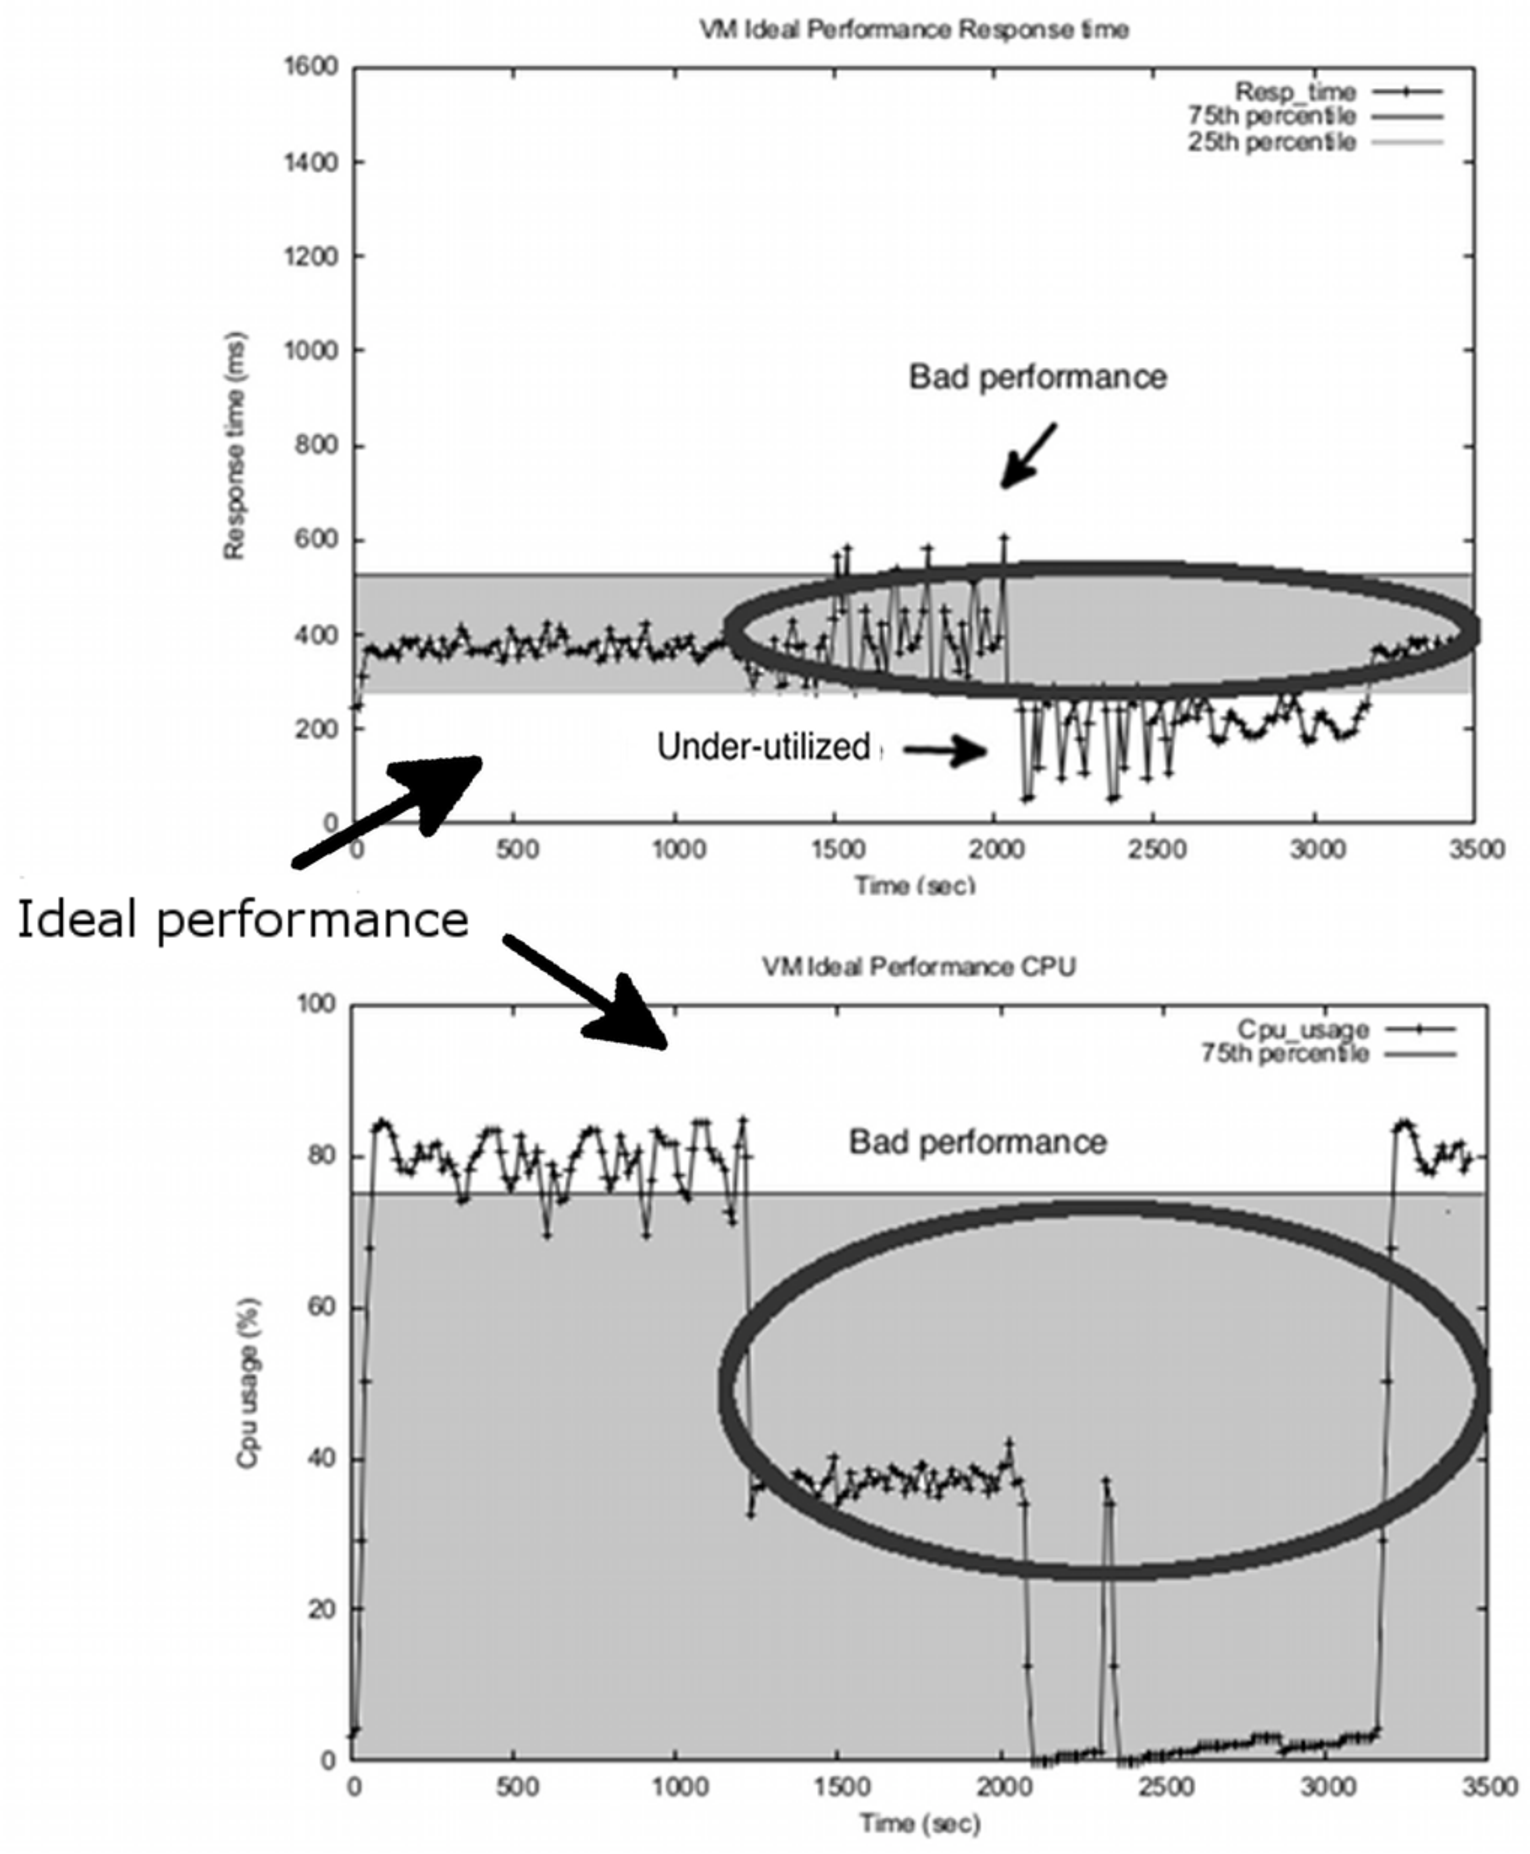
\includegraphics[height=8cm]{images/idealc1MediumRemark.pdf}
%		\captionof*{figure}{ \textbf{c1.medium}}
%		\vspace{-4mm}
%	\end{minipage}
%\caption{Profiling data and percentiles of m1.small and c1.medium EC2 instances.}
%\label{fig:vm_performance}
%\end{figure*}

\paragraph{Instance performance classification} The \emph{Profiler} classifies the different instance types depending on its computing capacity. Using the profiling smoothed data of each instance type (refer to Lines \ref{alg:throughput_start}-\ref{alg:throughput_end}), the Profiler computes a factor, named \emph{Ideal\_Throughput$_{inst}$}, as the amount of clocks required to serve a specific amount of requests (clocks/requests)  for one instance. In Equation~\ref{cpu_speed}, the \emph{\%CPU\_usage$_{inst}$} represents the average of percentage of cpu usage (clocks) and \emph{Num\_requests$_{inst}$} the average of request rate (requests) consumed during the last hour. Using this formula, we initially assume requests have the same complexity. Nevertheless, the \emph{request heterogeneity} will be taken into consideration when calculating the workload requirements, as explained in Section~\ref{workloadReq}.

%\fixme{Explain how we get the cpu usage.}


{\scriptsize
\begin{equation}\label{cpu_speed}
\begin{split}
\% CPU\_usage_{inst} = \dfrac{   \sum_{i=1}^N \big( \% cpu\_usage\_data_{i}  \big) } { N } \\
Num\_requests_{inst} = \dfrac{   \sum_{i=1}^N \big( req\_rate\_data_{i} \big) } { N } \\
Ideal\_Throughput_{inst} =\dfrac{ \bigg( \dfrac{\% CPU\_usage_{inst} } { 100 }  \bigg) } {  Num\_requests_{inst}   } 
\end{split}
\end{equation}
}

The \emph{Ideal\_Throughput$_{inst}$} factor gives an estimation of the optimized performance capacity of one VM instance when processing the current workload. This formula only works in the stable state when the system is not thrashing, and that we only measure it in the stable state using the percentiles. Based on the value of this factor per-instance, the \emph{Profiler} classifies the different instance-types based on its computing capacity when running an application. (See Lines \ref{alg:clas}-\ref{alg:end_clas}). The resulting classification gives an interesting feedback to the Scaler component, which is now able to identify the capacity of each instance type, and consequently to choose an optimal scaling plan. Note that, a lower value of the \emph{Ideal\_Throughput$_{inst}$} indicates a higher performance capacity. Initially, there are not instance profiles due to the lack of monitoring data, thereby the \emph{Scaler} uses the number of compute units per instance as a priori classification of their performance capacities. Our system only considers the compute units, but memory or network bandwidth can be also taken into consideration to classify the VM instances.

\vspace{2mm}
Finally, this profiling process allows to define a profile per instance type, thus facilitating the selection of an appropriate scaling plan that will satisfy the QoS requirements. Even though this profiling approach assumes that all the resources of the same type perform similarly, it can be easily extended to profile the allocated resources independently of its type. The performance of VM instances provided by current clouds is largely heterogeneous, even among instances of the same type~\cite{ec2Performance}.

%Similarly, the profiling data can be used independently of factors such as performance isolation in clouds or request heterogeneity to improve the accuracy of the scaling decisions.



\subsection{Scaling plan decision-making}

The discovery of a proper scaling plan is the most important and challenging phase in a provisioning system. It is responsible of the selection of an appropriate combination of resources that fulfills the QoS requirements.
% with the lowest operational cost. 

%This operation can become more laborious when running web applications, and therefore it has been barely addressed in the existing provisioning systems. Web applications are often a target of temporal traffic variations that may cause SLO violations having an impact in the user experience. Hence, the selection of an appropriate scaling plan becomes crucial to mitigate these penalties. 

%On the other hand, to boost the volume of customers, the user experience appears as a mandatory requirement in web applications contrary to budget cuts that may reduce the advantage over competitors.

To overcome this task, we should take into consideration three aspects: the workload requirements, the resource heterogeneity and the customer preferences. An exhaustive analysis of the current workload allows to identify the future demand that will determine the new configuration to use. This operation can become more laborious when running web applications due to their workload heterogeneity. On the other hand, cloud infrastructures offer a wide range of different hardware configurations that can be combined to better satisfy the requirements. Based on the customer preferences, the selection of one configuration or another can expose the application to availability or performance issues, specifically when handling workload variations or other traffic anomalies. Hence, the selection of an appropriate scaling plan becomes crucial to mitigate these penalties. 

%% Threshold fixed by the user



%\begin{figure*}[htb]
%	\begin{minipage}[b]{0.3\linewidth}
%		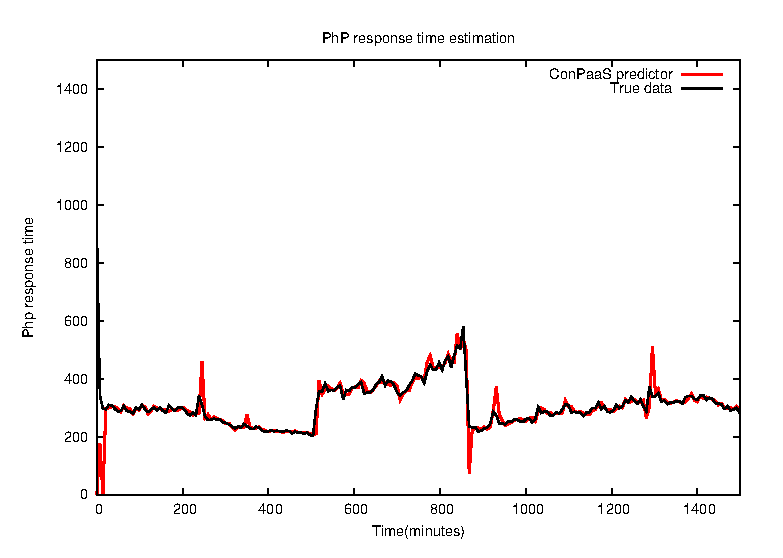
\includegraphics[height=4.5cm]{images/prediction_conpaas_6min.eps}
%		\vspace{-4mm}
%	\end{minipage}
%	\hfill
%	\begin{minipage}[b]{0.3\linewidth}
%		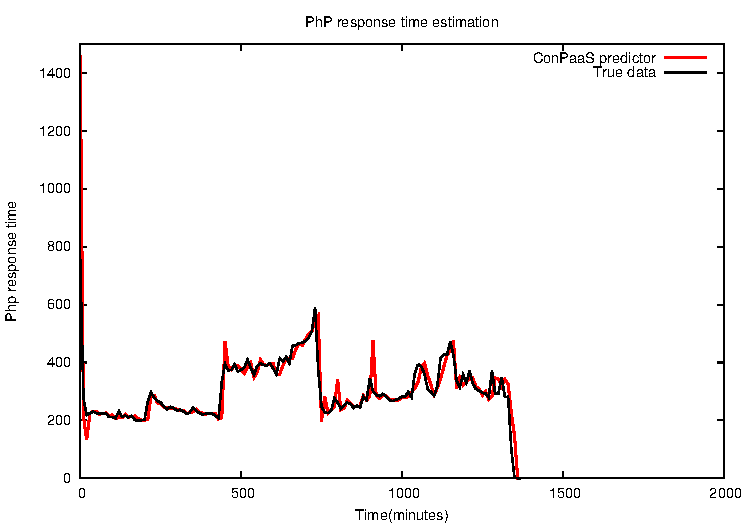
\includegraphics[height=4.5cm]{images/prediction_conpaas_10min}
%		\vspace{-4mm}
%	\end{minipage}
%	\hfill
%	\begin{minipage}[b]{0.3\linewidth}
%		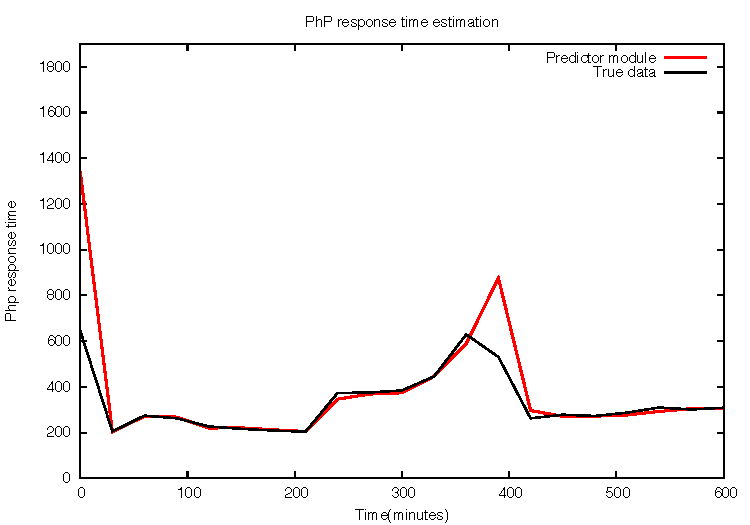
\includegraphics[height=4.5cm]{images/prediction_conpaas_30min}
%		\vspace{-4mm}
%	\end{minipage}
%\caption{ConPaaS Predictions, response times for 5min, 10min and 30min ahead.}
%\label{fig:vm_performance}
%\end{figure*}

%\subsubsection{Scaling strategy decision-making}



\subsubsection{Analysis of the workload requirements\label{workloadReq}}

Prior to any resource selection, the \emph{Scaler} has to measure the requirements of the current workload taken into account the traffic diversity of web applications. Traditional scaling systems gather monitoring data about the request volume or total percentage of cpu usage consumed to identify the workload requirements. However, the workload of web applications is highly heterogeneous being defined by sudden changes in the traffic as well as constantly-changing request mixes. As a consequence, our system computes the workload complexity considering both the total percentage of cpu usage and request rate served by the current scaling plan,  as factors that affect to the final response time. They provide enough information to detect the causes of a performance degradation in web applications. 

%In Equation~\ref{workload_complexity}, the \emph{$Workload_{complex}$} factor represents the complexity of the incoming traffic and includes degradations caused by operative system activities, low network performance, performance isolation or request heterogeneity. These degradations are omitted by individually analyzing the request rate or cpu usage consumed by all the allocated resources at any given time. Thus, the \emph{$Workload_{complex}$} is computed by using the sum of the cpu usage (denoted by \emph{$CPU\_usage_{i}$}) and the performance capacity of each allocated resource. The performance capacity is calculated as the average of the request rate served by each resource (denoted by $Num\_reqs_{i}$) and its ideal throughput (denoted by $Ideal\_Throughput_{inst_{i}}$). By using the ideal throughput instead of calculating the current throughput, the Scaler is able to measure how much the current workload is affecting the ideal performance pattern of a VM instance.

The \emph{workload complexity} is a factor that identifies how much the current workload is affecting the ideal performance pattern of the allocated resources. It identifies the complexity of the incoming traffic and includes degradations caused by operating system activities, low network performance, performance isolation or request heterogeneity. These degradations affect the performance and are often omitted by individually analyzing the request rate or cpu usage consumed by the allocated resources. 

To calculate the \emph{workload complexity} (denoted by \emph{$Workload_{complex}$}), we first analyzes the monitoring data gathering the request rate (denoted by $Num\_reqs\_server_{i}$) and total percentage of cpu usage (denoted by \emph{$\%CPU\_usage\_server_{i}$}) consumed by the allocated \emph{N} resources during the monitoring window. Secondly, unlike the \emph{\%CPU\_usage$_{inst}$},  we calculate the expected usage of CPU of each resource \emph{i} (denoted by \emph{CPU\_usage\_expected$_{i}$} ) using its current request rate (denoted by $Num\_reqs\_server_{i}$) and its \emph{optimized throughput} (denoted by $Ideal\_Throughput_{inst_{i}}$). By doing so, we are able to include into the \emph{$Workload_{complex}$} all the degradations that affect the ideal performance of the application. Finally we compute the \emph{$Workload_{complex}$} factor using the sum of cpu usage consumed to handle the current workload and the sum of expected cpu usage of all the resources, as illustrated in Equation~\ref{workload_complexity}.


%\fixme{We could include in the Equation some additional information to define each factor.}

{\scriptsize
\begin{equation}\label{workload_complexity}
\begin{split}
CPU\_usage\_expected_{i} =  Num\_reqs\_server_{i}  * Ideal\_Throughput_{inst_{i}} \\
Workload_{complex}  = \dfrac{ \bigg(  \dfrac{ \sum_{i=1}^N \%CPU\_usage\_server_{i} } {100} \bigg) }  {  \sum_{i=1}^N  CPU\_usage\_expected_{i}     } = \dfrac{ \ (clocks) }  {  (clocks) }
\end{split}
\end{equation}
}

Additionally, the future service demand of the application, in terms of total percentage of cpu usage and request rate consumed by the resources, can be estimated by the \emph{Predictor} component for the next monitoring windows (in our experiments 30min). This enables to select in advance a scaling strategy that will handle future fluctuations in the workload, and thereby saving cost. However, a detailed explanation of how the \emph{Predictor} component estimate future workload requirements is not in the scope of this paper.

%Additionally, the future service demand of the application, in terms of total percentage of cpu usage and request rate consumed by the resources, can be estimated by the \emph{Predictor} component for the next monitoring windows (in our experiments 30min). This enables to select in advance a scaling strategy that will handle future fluctuations in the workload, and thereby saving cost. As an example in Figure~\ref{fig:forecast}, the \emph{Predictor} shows the forecast values for the resource requirements during the next 30 minutes offering an acceptable level of accuracy. To calculate the precision of the forecasting results, we used metrics such as PRED(25)~\cite{jorgensen_experience_1995} and Mean Absolute Percentage Error (MAPE)~\cite{islam_empirical_2012} that obtained values 0.904 and 0.109 respectively. By definition, PRED(25) values closer to 1.0 and MAPE values closer to 0.0 indicates a better fit of the prediction model; thus indicating correct prediction rate of our forecasting results.

% An aspect to notice is that the forecasting results never under-provision the system avoiding the generation of unnecessary SLO violations.

% PRED(25) value closer to 1.0 indicates a better fit of the prediction model.
% A lower value of MAPE implies a better fit of the predciction model; thus indicating superior prediction accuracy.
% PRED(25) = num. observations with relative error <= 25% / num observations = 19/21 ... and MAPE = 1/n sum( |y_pred - y| /y )

%\begin{figure}[t]
 % \begin{center}
 %   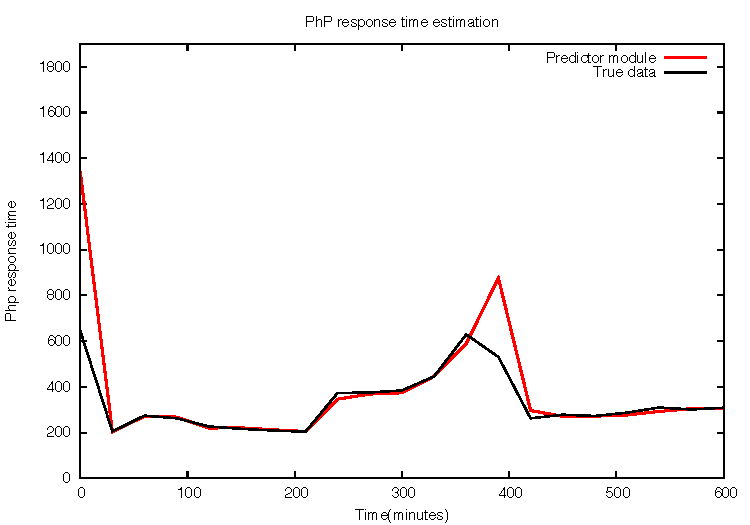
\includegraphics[width=0.8\linewidth,height=5cm]{images/prediction_conpaas_30min}
 % \end{center}
%\vspace{-3mm}
%  \caption{Predictor component: forecasting results 30min ahead.}
%  \label{fig:forecast}
%\end{figure}


\subsubsection{Calculating the different scaling plans}

To decide which type and amount of VM instances to add or release, the \emph{Scaler} uses an optimal decision tree that facilitates the discovery of all the possible scaling strategies. By going through this tree, our system evaluates all the possible resource combinations using horizontal scaling operations (out, back). As shown by Figure~\ref{fig:scalingTree}, in the scaling decision tree, each node represents each type of hardware configuration offered by a cloud infrastructure, where the nodes linked by a straight line represent the current scaling strategy. While the branches, denoted by a dotted line, define all the possible resource combinations to provision. 

\begin{figure}[t]
  \begin{center}
    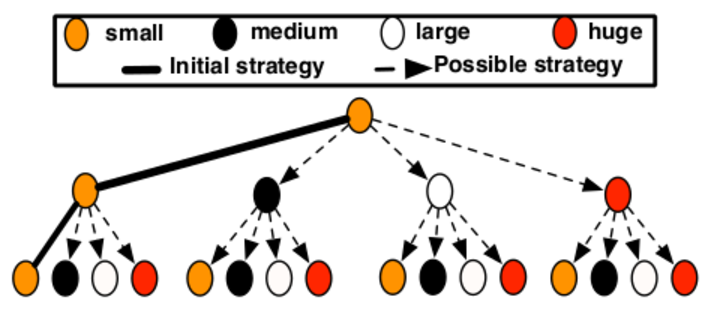
\includegraphics[width=0.7\linewidth,height=2.5cm]{images/optimalTree_initial}
  \end{center}
\vspace{-3mm}
  \caption{Example of a decision tree created from an existing resource combination.}
  \label{fig:scalingTree}
\end{figure}

During the selection process of possible scaling strategies, the \emph{Scaler} uses Equation~\ref{resource_combination} to compute how a strategy will distribute the current workload across the different resources taken into account their performance capacities.  Equation~\ref{resource_combination} defines a factor, called \emph{RU\_Strategy}, that determines the resource utilization of a strategy when handling the current or future workload (depending on how the workload requirements were obtained). According to that, the \emph{Scaler} selects a strategy that uses \emph{N} resources to distribute the \emph{$Num\_reqs_{total}$} (total requests served by the current resources or estimated by the \emph{Predictor}) with a workload complexity \emph{$Workload_{complex}$} across \emph{N} instance types with different optimized throughputs \emph{$Ideal\_Throughput_{inst_{k}}$}. As a function of the \emph{$Ideal\_Throughput_{inst}$} and \emph{$Num\_reqs_{total}$}, the \emph{$RU\_Strategy$} measures the resource utilization (clocks) to process the current workload when using a specific resource combination.

%When processing the current workload, to decide which resources to include in the scaling plan,  the \emph{Scaler} uses the following formula: 

%This formula determines the CPU usage consumed to process the current workload when using a specific resource combination (denoted by \emph{$CPU_{strategy}$}). Note that, CPU usage provides enough feedback about the performance capacity, as it is a function of the request complexity  and number of served requests. 

%To calculate the different combinations of VM instances that enforce the performance requirements, we used the next


{\scriptsize
\begin{equation}\label{resource_combination}
\resizebox{\linewidth}{!}{
\begin{tabular}{l@{}l@{}}
{\small RU\_Strategy = Resource utilization of the strategy } \\ \\
$RU\_Strategy_{i} = \dfrac{ \sum_{k=1}^N \bigg( \bigg( \dfrac{ Num\_reqs_{total} } {N}  * Workload_{complex} \bigg) * Ideal\_Throughput_{inst_{k}} \bigg) }  {N}$
\end{tabular}
%\\ {\small \textit{ If } CPU\_usage_{strategy} \leqslant CPU\_max_{SLO} }
}
\end{equation}
}



%As an example, Figure~\ref{fig:scalingTree} shows three scaling plans that propose three different resource combinations: (left) a strategy is selected by adding two new \emph{small} instances, (center) a strategy proposes to replace one \emph{small} instance by one \emph{large}, and (right) both operations are combined by replacing one \emph{small} instance by one \emph{medium} and then adding one \emph{small}. 

Note that, the search space of possible strategies can be as large as the number of available hardware configurations, and allocated resources of the current scaling plan. It makes it difficult to find the best resource combinations in a reasonable short period of time, so that the \emph{Scaler} defines two policies to filter the pausibles strategies based on the following criteria:


\begin{itemize}

\item Define the maximum resource utilization consumed  by a strategy when processing a particular workload (denoted by \emph{$Max\_RU\_Strategy$}). It limits the number of possible plans where \emph{$RU\_Strategy_{i} \leq Max\_RU\_Strategy$}. \emph{$Max\_RU\_Strategy$} specifies the maximum resource utilization at which the application starts to experience SLO violations or over-utilization of the resources. Its value can be extracted either from the Amazon EC2 recommendations for the maximum percentage of CPU usage (CPU usage always lower than 75\%), or based on the monitoring data (gathered by the monitoring engine) at which the application starts to experience SLO violations. As a result of this policy, the proposed scaling plans optimizes the current performance below values causing performance degradations. 

%can be calculated either based on the Amazon EC2 recommendations ( CPU values always lower than 75\%), or based on the CPU values at which the application starts to experience SLO violations (or performance degradations). 

\item Include a cost policy to avoid choosing wasteful scaling strategies. Considering the pricing model of cloud providers that charges users on a per-hour basis, the \emph{Scaler} includes a cost policy that rejects strategies releasing resources which have been recently started ( 5min $<$ time to the end of its hour $<$ 20). The \emph{Scaler} releases resources which are closed to the hour are free under the cloud pricing model, and there is no gain from terminating them before this hour price boundary.

\end{itemize}

These two policies avoid to trigger new scaling actions in short time intervals (e.g. within less than one hour), and consequently reduce the operational cost. 


%As an example of the selection process
\noindent\textbf{Example:} Figure~\ref{fig:scalingTreeSelection} shows three possible scaling plans obtained by using our decision tree and Equation~\ref{resource_combination} (denoted by \emph{Eq(3)}) over the initial strategy illustrated in Figure~\ref{fig:scalingTree}. This initial resource combination is composed of three \emph{small} instance types which are not enough to handle the current workload. Using this strategy as reference and horizontal scaling operations, our algorithm adds and/or releases resources (leafs to the tree) as long as the resulting \emph{$RU\_Strategy$} (calculated for the new resource combination) is lower than \emph{$Max\_RU\_Strategy$} and do not propose to release resources recently added. As a result, three plans (trees) are proposed using different resource configurations and satisfying the performance requirements to handle the workload. This discovery process stops when all the possible combinations have been proved or there are not more combinations satisfying the aforementioned filtering criteria. 



\begin{figure}[t]
  \begin{center}
    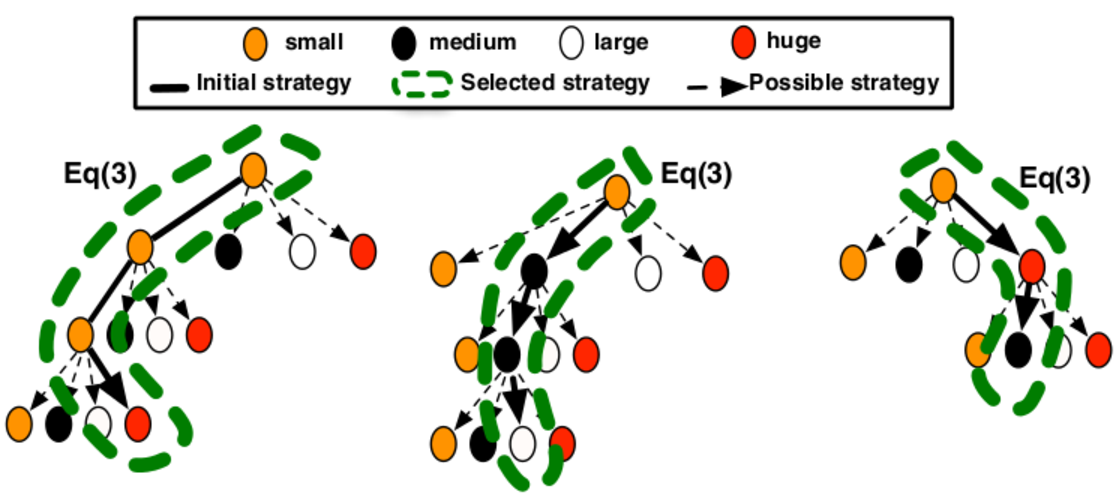
\includegraphics[width=0.7\linewidth,height=3cm]{images/optimalTree_selection}
  \end{center}
\vspace{-3mm}
  \caption{Example of three selected scaling plans that satisfy the filtering criteria.}
  \label{fig:scalingTreeSelection}
\end{figure}



In summary, using the Equation~\ref{resource_combination}, the Scaler is able to answer to the question \emph{"How many and which instance-types to provision?"}.

%is calculated using the Profiler component and will variate depending on the type of vm instance used in the strategy. 

\subsubsection{Selecting the optimal scaling plan}

%To refine this search process according to the final goal and adapted to the customer preferences (user experience), the Scaler provides three classes of SLA agreements in function of the type of customer. These three classes of customers namely, gold, silver and bronze minimize the SLA violations with a different infrastructure cost. Accordingly, a gold customer pays more in order to get the best service at the cost of some extra over-provisioning. A silver customer gets good availability while a bronze customer obtains a reduced, but acceptable, SLA fulfillment but with very little over-provisioning.

%they are classified based on their infrastructure cost and degree of SLO fulfillmen

Once the \emph{Scaler} obtains a list of filtered scaling strategies, it computes the cost of applying each possible strategy how the cost incurred by its SLO fulfillment degree and the infrastructure cost. The infrastructure cost (denoted by \emph{Infra\_cost}) specifies the cost required to provision a scaling plan for the next hour. While the SLO fulfillment degree (denoted by \emph{SLO\_fulfillment}) indicates the vulnerability of a scaling plan to experience SLO violations. 

As defined in the Equation~\ref{strategy_cost}, the \emph{SLO\_fulfillment} cost is calculated given the \emph{$RU\_Strategy_{i}$} of a strategy \emph{i} and the \emph{$Max\_RU\_Strategy$}. Obviously, higher values in the \emph{$RU\_Strategy$} imply an increment in the probability of having SLO violations under traffic spikes, so the \emph{SLO\_fulfillment} will increase as well. 

%As defined in the Equation~\ref{strategy_cost}, the \emph{slo\_fulfillment} cost is calculated given the percentage of \emph{$CPU_{strategy}$} and the \emph{$CPU_{SLO}$}, multiply by a SLO penalty (in \$)  pre-established between the customer and provider. Obviously, higher values in the percentage of \emph{$CPU_{strategy}$} imply an increment in the probability of having SLO violations under traffic spikes, so the \emph{slo\_fulfillment} will increase as well. 

%Therefore, according to the customer preferences, the Scaler can select one strategy with the lowest, highest or medium cost.

{\scriptsize
\begin{equation}\label{strategy_cost}
\begin{split}
Infra\_cost_{i} = \sum_{k=1}^N \big( instance\_price_{k} \big) \\
%slo\_fulfillment =  \bigg( \dfrac{ CPU_{strategy} } {CPU_{SLO}} \bigg) * SLO penalty \\
SLO\_fulfillment_{i} =  \bigg( \dfrac{ RU\_Strategy_{i} } {Max\_RU\_Strategy} \bigg)  \\
Cost\_strategy_{i} = \dfrac{  SLO\_fulfillment_{i}  } {Infra\_cost_{i}}
\end{split}
\end{equation}
}

%\fixme{I could omit the use of the SLO penalty, as it is a constant in my experiments. Instead I could say that the system adapts to the user needs.}

The criteria for the selection of the optimal scaling plan is configurable, and thereby it can adapted to the customer preferences. For instance, large enterprises need to provide high availability and performance to their clients, disposing of a generous budget for such a mission. Therefore, based on the customer-tradeoff between performance/cost, the \emph{Scaler} component will choose to provision one scaling plan or another depending on the value of its \emph{Cost\_strategy}. 

To facilitate the specification of the performance/cost preferences to the customers, our system provides different pre-defined criteria that adapt the scaling decisions to these requirements. These selection criteria are defined thanks to a \emph{metal classification} that classifies  the different type of customers based on their performance/cost preferences. Initially, we define three different classes of customers following this \emph{metal classification}. These three classes of customers namely, Gold, Silver and Bronze minimize the SLA violations with a different infrastructure cost. 

\begin{itemize}
\item A \emph{Gold customer} identifies those customers that pay more in order to get the best service at the cost of some extra over-provisioning. The \emph{Scaler} then selects the strategy that has the highest \emph{Cost\_strategy}.
\item A \emph{Silver customer} includes those customers that prefer to get good availability but with a reasonable operational cost. As such, the \emph{Scaler} calculates the median \emph{Cost\_strategy} of all the possible strategies, and uses it as the strategy to provision.
\item A  \emph{Bronze customer} represents those customers who are willing to obtain a reduced, but acceptable, SLO fulfillment but with very little over-provisioning; and thereby a low operational cost. The \emph{Scaler} uses as the optimal strategy that one with the lowest \emph{Cost\_strategy}.

\end{itemize}

In our experiments, we will use this \emph{metal classification} to show the benefits/drawbacks by selecting different scaling plans based on the class of customer.
% when handling sudden workload variations.

%To classify the provisioning decisions based on the tradeoff between performance/cost of the customer preferences, we define three different classes of customers following a medal classification. These three classes of customers namely, gold, silver and bronze minimize the SLA violations with a different infrastructure cost. For instance, a gold customer pays more in order to get the best service at the cost of some extra over-provisioning. A silver customer gets good availability while a bronze customer obtains a reduced, but acceptable, SLO fulfillment but with very little over-provisioning. 



%Moreover, \emph{$SLO_{penalty}$} can be also used as a criteria for the selection of the most appropriated strategy according to some requirements.

%To decide which type of instance to release, the Scaler uses a conservative algorithm that releases the resources with the lowest utilization by analyzing their monitoring data. Similarly, a cost policy was also included for avoiding to choose wasteful scaling decisions. Considering the pricing model of cloud providers that charges users on a per-hour basis, the Scaler includes a cost policy that rejects strategies releasing vm instances which have been recently started ( 5min < time to the end of its hour < 20). Scaler releases resources which are closed to the hour are free under the cloud pricing model, and there is no gain from terminating them before this hour price boundary.

%A complete point of view of the whole scaling flow is shown in Figure~\ref{autoScalingFlow}.

%\begin{figure}[htb]
%  \begin{center}
 %   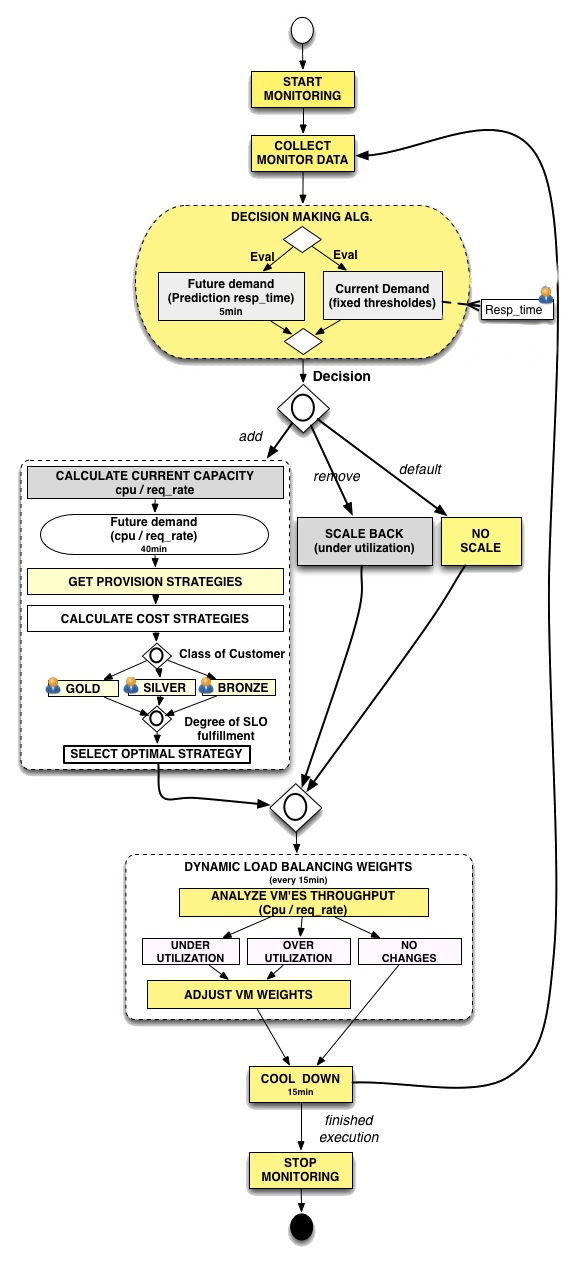
\includegraphics[width=\linewidth]{images/NewAutoScalingFlow}
%  \end{center}
%\vspace{-5mm}
%  \caption{Auto scaling flow.}
%  \label{autoScalingFlow}
%\end{figure}


%\subsection{Dynamic load balancing weights } 


%The problem we consider here is again the heterogeneity of cloud platforms.
%Independently of its size, different VM instances from the same cloud might have different performance
%characteristics, even when their specifications from the cloud vendor are 
%the same~\cite{ec2Performance}. This issue can be addressed through various 
%load balancing techniques, like assigning weights to the backend servers or 
%taking into account the current number of connections that each server 
%handles. Furthermore, the performance behavior of the virtual servers may 
%also fluctuate, either due to changes in the application's usage 
%patterns, or due to changes related to the hosting of the virtual servers 
%(e.g., VM migration).


%\begin{figure}[t]
 % \begin{center}
 %   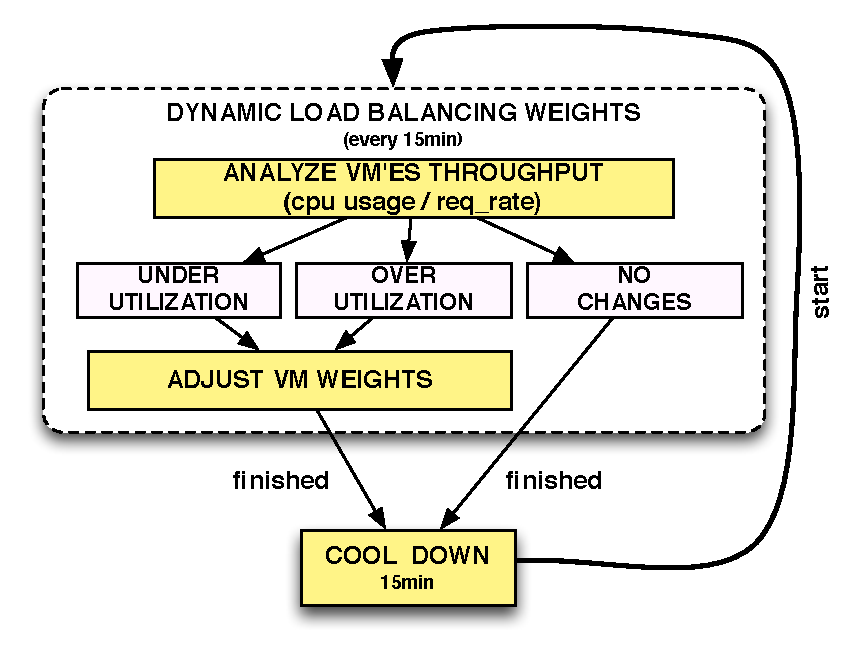
\includegraphics[height=4cm]{images/load_balancing}
%  \end{center}
%\vspace{-3mm}
%  \caption{Weighted load balancing flow.}
%  \label{fig:load_balancing}
%\end{figure}


%In order to address these issues, the Scaler implemented a weighted 
%load balancing system in which the weights of the servers are 
%periodically re-adjusted automatically, based on the monitoring data.  
%This method assigns the same weight to each backend server at the 
%beginning of the process. As illustrated in Figure~\ref{fig:load_balancing}, the weights are then %periodically
%adjusted (in our experiments, using a window of $\sim$ 15min) proportionally 
%with the difference among the average of percentage of cpu usage and request rate served by the servers 
%during this time interval. By adding this technique to our autoscaling system, 
%the workload can be dynamically and proportionally distributed across the provisioned VM instances depending on their performance capacities.

%we noticed a performance improvement when running the benchmarks, as discussed in the following.



